\chapter{REVIEW OF RELATED LITERATURE}
{\baselineskip=2\baselineskip
 This chapter focuses on related studies or projects that have provided additional relevant information to the proponent. Section 2.1 presents the theoretical background related to machine learning and mechatronics. Section 2.2 specifies the concept of how the system will classify the eggplants by class based on surface defects, color homogeneity, and shape. Section 2.3 presents a review of literature related to the design of employing machine learning and mechatronic integration in agricultural automation for image-based inspection and mechanical sorting applications. Collectively, these reviewed literatures support the concept presented in this study. 

%-----------------------------------------------------------------------------------------------------------------------
\section{Theoretical Background}
The development of an automated eggplant grading system is fundamentally grounded in the integration of theoretical paradigms of computational intelligence and mechanical control. This framework draws from the convergent disciplines of machine learning and mechatronics to create a cyber-physical system capable of perceiving, deciding, and acting. The following subsections detail the core theories that underpin the image analysis, classification, and physical sorting mechanisms of the proposed system.

\begin{figure}[h]
	\centering
	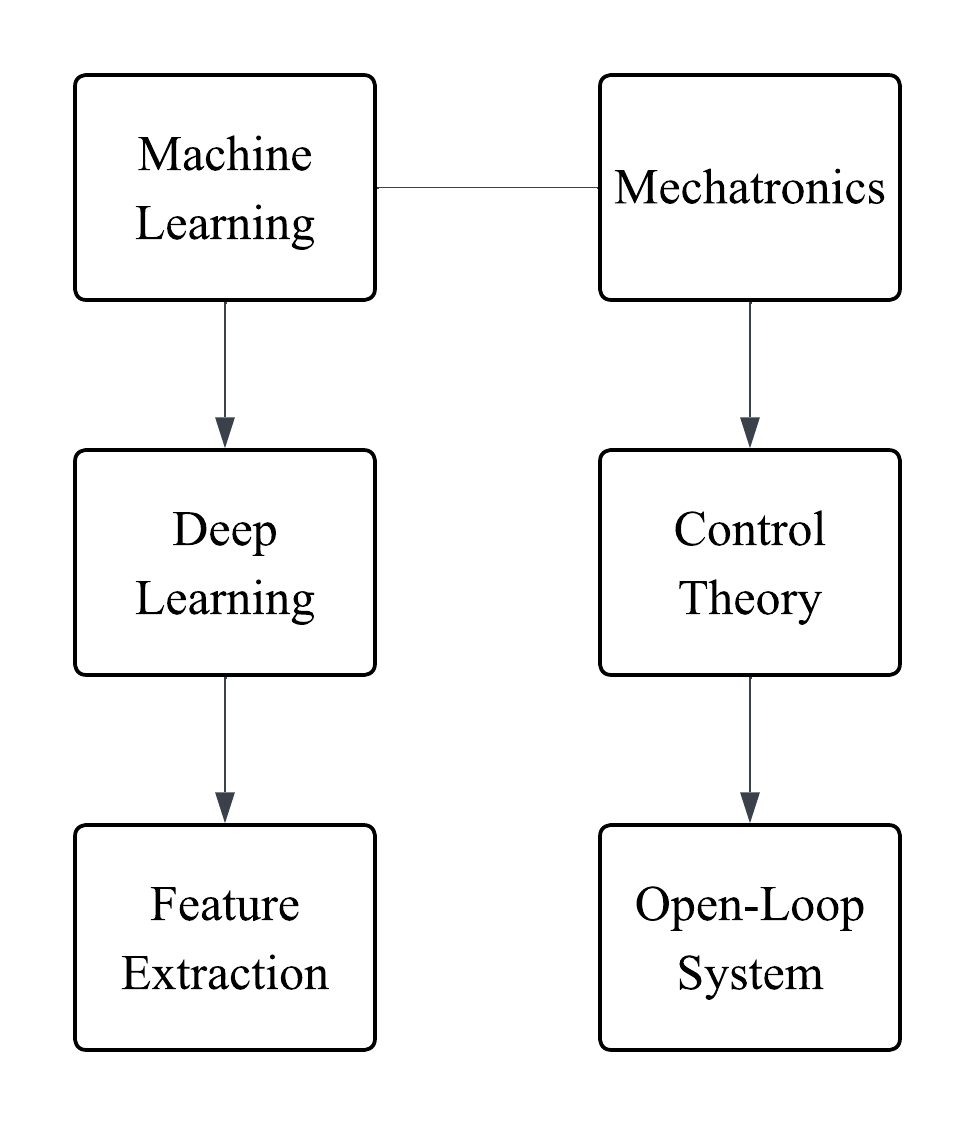
\includegraphics[height=0.4\textheight]{figures/theoreticaldiagram}
	\caption{Theoretical Framework}
	\label{fig:theoreticalframework}
\end{figure}

The development of an automated eggplant grading system is fundamentally grounded in the integrated theoretical paradigms of computer vision, deep learning, and mechatronics. The entire process can be conceptualized through a sequential computer vision pipeline, which moves from image acquisition to physical actuation \citep{szeliski2022computer}. This pipeline begins with the digital image formation theory, where a camera sensor captures light reflectance from objects on a conveyor belt, a common setup in food process engineering \citep{dougherty2020digital}. The stability and quality of this initial stage are paramount, as controlled, diffuse illumination is critical to minimize specular reflections and shadows that can obscure critical features like color and surface defects, thereby ensuring consistent input for subsequent algorithmic processing.

Following acquisition, image pre-processing theories are applied to enhance data quality and standardize inputs. This involves digital signal processing techniques such as noise reduction using Gaussian or median filters \citep{kumar2020comparative} and, crucially, color space transformation. Converting images from the default Red-Green-Blue (RGB) space to Hue-Saturation-Value (HSV) or \textit{CIEL*a*b*} is a well-established step in agricultural product inspection \citep{khan2024intelligent}. The theoretical underpinning for this conversion lies in the decoupling of color information (chrominance) from intensity (luminance) in these spaces, making the extracted color features more robust to minor variations in lighting conditions, which is essential for accurate color-based grading.

The core of the system resides in the theoretical distinction between traditional machine learning and deep learning for feature extraction. Traditional approaches are based on manual feature engineering, drawing from image processing and pattern recognition theory to hand-craft descriptors for color (e.g., histograms, mean values), shape (e.g., aspect ratio, roundness, area), and texture (e.g., using Gray-Level Co-occurrence Matrix (GLCM) or Local Binary Patterns (LBP)) \citep{haralick2007textural,ojala2002multiresolution}. In contrast, deep learning, specifically Convolutional Neural Network (CNN) theory, posits that models can automatically learn a hierarchical representation of features directly from raw pixel data \citep{lecun2015deep,goodfellow2016deep}. The lower layers of a CNN learn generic features like edges and corners, while deeper layers synthesize these into complex, task-specific features relevant to defect identification, thereby eliminating the need for manual feature design.

For the classification task itself, the theoretical models diverge. Machine learning classifiers operate on the principles of statistical learning theory, finding optimal hyperplanes to separate classes or constructing ensembles of decision trees, respectively, based on the handcrafted features \citep{hearst1998support,breiman2001random}. Conversely, an end-to-end deep learning model uses a fully connected output layer with a normalized exponential function (also known as \textit{Softmax}) to perform classification based on the high-level features it learned itself. The theoretical advantage of CNNs is their superior ability to model complex, non-linear relationships in visual data, a capability that has been demonstrated to outperform traditional methods in numerous agricultural applications \citep{bharman2022deep}.

The integrity of any supervised learning system is dependent upon the quality of its labeled dataset. The establishment of a reliable ground truth is a theoretical problem rooted in psychometrics and expert systems. The grading labels for the eggplant images must be derived from standardized agricultural protocols, such as those provided by the United States Department of Agriculture (USDA) or equivalent bodies, which define quality classes based on size, color uniformity, and defect tolerances \citep{USDA2013EggplantStandards}. Locally, the project will utilize the criteria defined by the Philippine National Standard (PNS), and Bureau of Agricultural and Fisheries Product Standards (BAFPS) (specifically the PNS/BAFPS 52:2007), which classifies eggplants into Extra Class, Class I, and Class II based on visual quality, size, and defect tolerances \citep{PNSBAFPS522007_Eggplant,BAFS2019PhilGAP}. To ensure scientific rigor, the concept of inter-rater reliability, often measured by Cohen’s Kappa statistic ($\kappa$), must be applied to quantify the agreement between human experts who label the dataset, thereby validating the consistency of the training labels \citep{mchugh2012interrater,he2022cohens}.

The closed-loop system theory integrates the digital classification with physical actuation. The decision output from the classification model (e.g., a specific grade) is transmitted via a software-to-hardware interface to a Programmable Logic Controller (PLC) or microcontroller \citep{bolton2015programmable}. This triggers a mechatronic actuator, such as a pneumatic pusher or a servo-controlled diverter, which physically sorts the eggplant into its designated bin on the conveyor line. This final stage embodies the principle of cyber-physical systems, where computational intelligence directly controls a physical process to achieve full automation, replicating and potentially surpassing human grading efficiency \citep{lee2008cyber,zhang2022advancements}.